
\chapter{Architecture}
\label{sec:treehousearch}
 
\section{Background}
%Architectural structures   

\section{Elements for Tree-Based Architecture} 
\label{sec:archelements}
 
 
%nog iets moois hiervoor 
In this section we present the set of elements we use for the construction of our treebased architecture. We will first introduce the elements in a broad sense, followed by detailed descriptions of methods to construct each of the elements procedurally. 
 
 
\subsection{The Element Vocabulary}
We established a set of architectural elements we believe are vital for the generation of tree-based architectural structures. The elements are the following: 
\begin{enumerate}
\item platform
\item housing
\item bridge 
\item stairs
\end{enumerate} 



\begin{figure}[ht]
\centering
\subfigure[Platform]{
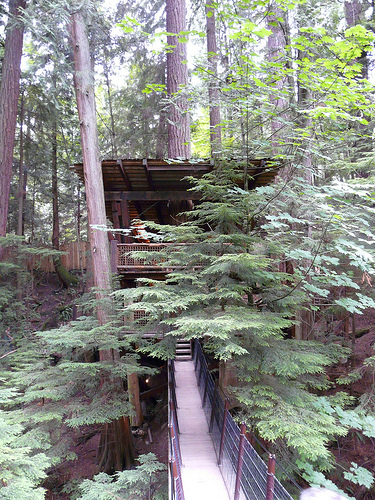
\includegraphics[width=50px]{images/platform.jpg}
\label{fig:subfig1}
}
\subfigure[House]{
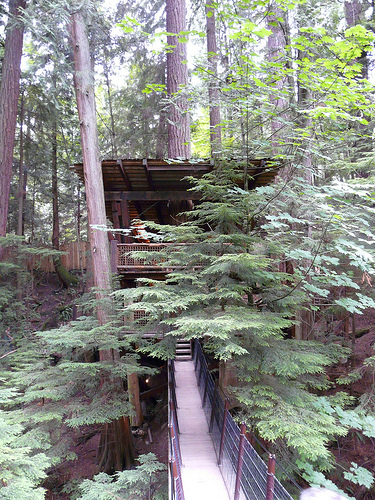
\includegraphics[width=50px]{images/house.jpg}
\label{fig:subfig2}
}
\subfigure[Bridge]{
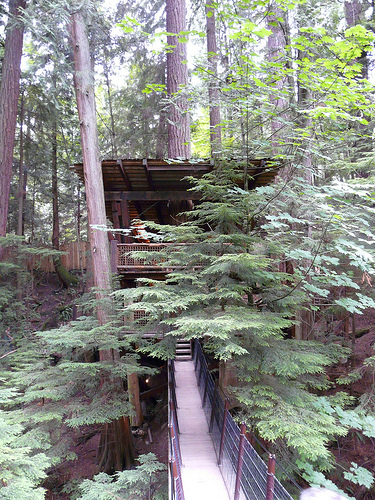
\includegraphics[width=50px]{images/bridge.jpg}
\label{fig:subfig3}
}
\subfigure[Stairs]{
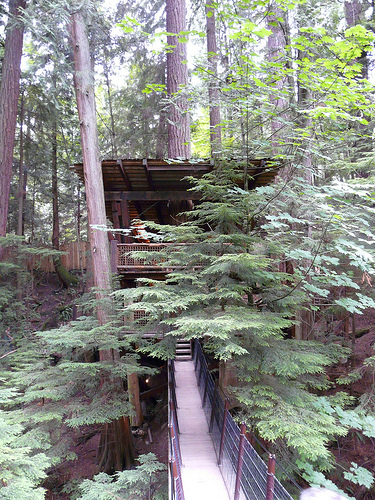
\includegraphics[width=50px]{images/stairs.jpg}
\label{fig:subfig3}
}
\label{fig:archElements}
\caption[Architectural Elements Vocabulary]{Caption of subfigures \subref{fig:subfig1}, \subref{fig:subfig2} and \subref{fig:subfig3}}
\end{figure}



\subsection{Combining Elements} 

We construct an architectural structure by combining the elements we have in our element vocabulary.
In order to construct logical combinations we need to define for each elements how it can be joined with other elements
in our vocabulary.
 
\subsection{Platforms}
\label{sec:platform}
 

 

\subsection{Housing}
\label{sec:building}
 

\subsection{Bridges}
\label{sec:bridges}
 

\subsection{Stairs}
\label{sec:stairs}
  
 
%introductie van alle elementen


 I want to implement this as a graph traversing algorithm
 (using the Boost graph library)
 
 
\section{Scenarios}
\label{sec:scenarios}

Here we define one or more scenarios for meaningful architectural planning with a forest scene.
The scenarios that are proposed here will be transformed to rules, heuristics and parameters in 
the next section 
	
	
\subsection{Single Family Retreat}
\subsection{Tree Village}
\subsection{Fantasy Tree City}


\section{Formalizing the Scenarios}

From the scenarios I discussed in the previous section we can extract a set of parameters and goals for our algorithm.
 
\section{Structure Planning}
\label{sec:PlanningAlgorithm} 
  
 Using the scenarios and architectural elements we have defined in the previous section we will formulate our planning algorithm now.
 I will first introduce the planning algorithm informally followed by a more formal approach.
      
 
 	 
 
%\begin{algorithm}
%\caption{The planning algorithm}
%\begin{algorithmic}
%\IF {$i\geq maxval$} 
%        \STATE $i\gets 0$
%\ELSE
%        \IF {$i+k\leq maxval$}
%                \STATE $i\gets i+k$
%        \ENDIF
%\ENDIF 
%\end{algorithmic}
%\end{algorithm}


 \subsection{Alternative approaches}
 